%!TEX root = Slic3r-Manual.tex
\section{Simple Mode} % (fold)
\label{sec:simple_mode}
\index{simple mode}

Slic3r has two modes of operation, Simple and Expert. These may be chosen from the \texttt{Preferences} window (found under the \texttt{File} menu).

\begin{figure}[ht]
\centering
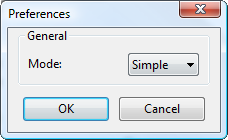
\includegraphics[width=0.3\textwidth]{simple_mode/preferences_general.png}
\caption{Preferences.}
\label{fig:preferences_general}
\end{figure}

Simple mode offers a reduced set of options, enough for the beginner to get started with.  Expert mode give more control over how Slic3r produces the G-code and will be looked at later.

\subsection{Print Settings}
\index{Print Settings}

The \texttt{Print Settings} tab provides the opportunity to change settings related to the actual print.  Whereas the other tabs are changed rarely, the settings on this tab will be modified regularly, possibly for each model printed.

\begin{figure}[ht]
\centering
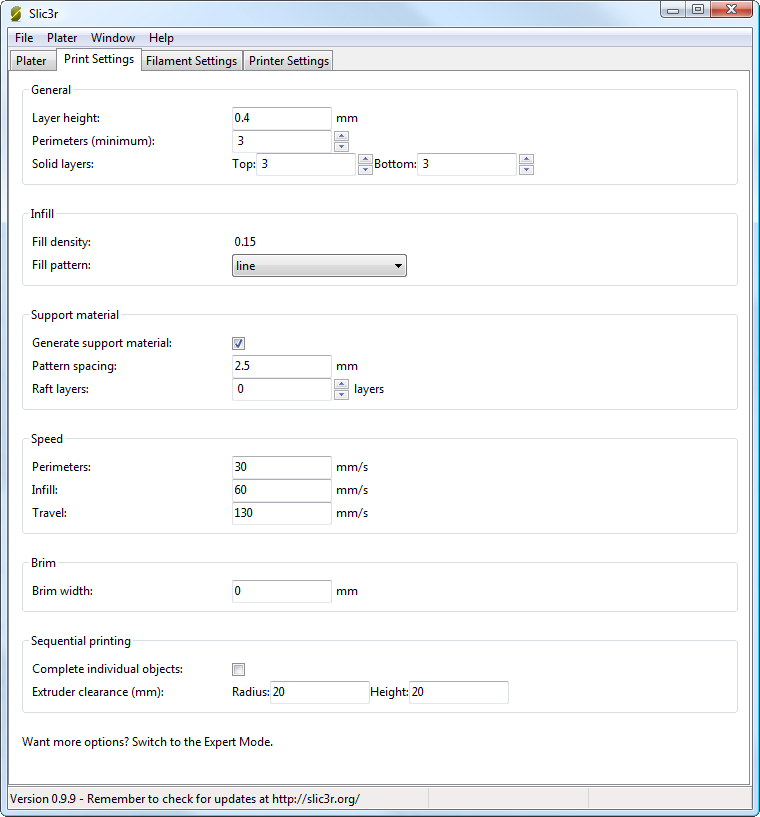
\includegraphics[width=\textwidth]{simple_mode/simple_mode_print_settings.png}
\caption{Simple Mode: Print Settings.}
\label{fig:simple_mode_print_settings}
\end{figure}

\paragraph{General.} % (fold)
\label{par:simple_general}
\index{Print Settings!Layer height}

\texttt{Layer height} is the thickness of each layer, and it is the step along the vertical axis taken before extruding a new layer atop the previous one.  There are several factors that influence how high each layer should be:
\begin{itemize}
	\item \textbf{Desired resolution}  - Lower layer height should result in prints with less noticeable ribs or bands, as each layer is smaller.  Aesthetics plays a role here, but also the type of model, for example, a mechanical part may not need such a high resolution finish, whereas a presentation piece may do so.
	\item \textbf{Print speed}  - Shorter layers will result in smoother prints but each print will take longer, simply because the extruder must trace the pattern more times.  A later goal will be to strike a balance between layer height, the speed of the printer, and the quality of the resulting print.
\end{itemize}
\index{Print Settings!Perimeters}
\texttt{Perimeters} defines the minimum number of vertical shells (i.e. walls) a print will have.  Unless the model requires single width walls it is generally recommended to have a minimum of two perimeters as this gives some insurance that if a section of the perimeter is not printed correctly then the second perimeter will help cover it.

\index{Print Settings!Solid layers}
The upper and lowermost layers that sandwich the model are filled with a \texttt{Solid layers} pattern.  For the bottom layers the important factor to consider is how the surface will look should there be a mistake whilst laying down the first layer, and for this reason it is recommended to have at least two bottom layers.

A similar consideration is required for the top layers.  Because the intermediate layers are likely to be filled with a pattern set less than 100\% then the covering layers will have to bridge this pattern and this can require more than one pass to cover completely.

\begin{figure}[H]
\centering
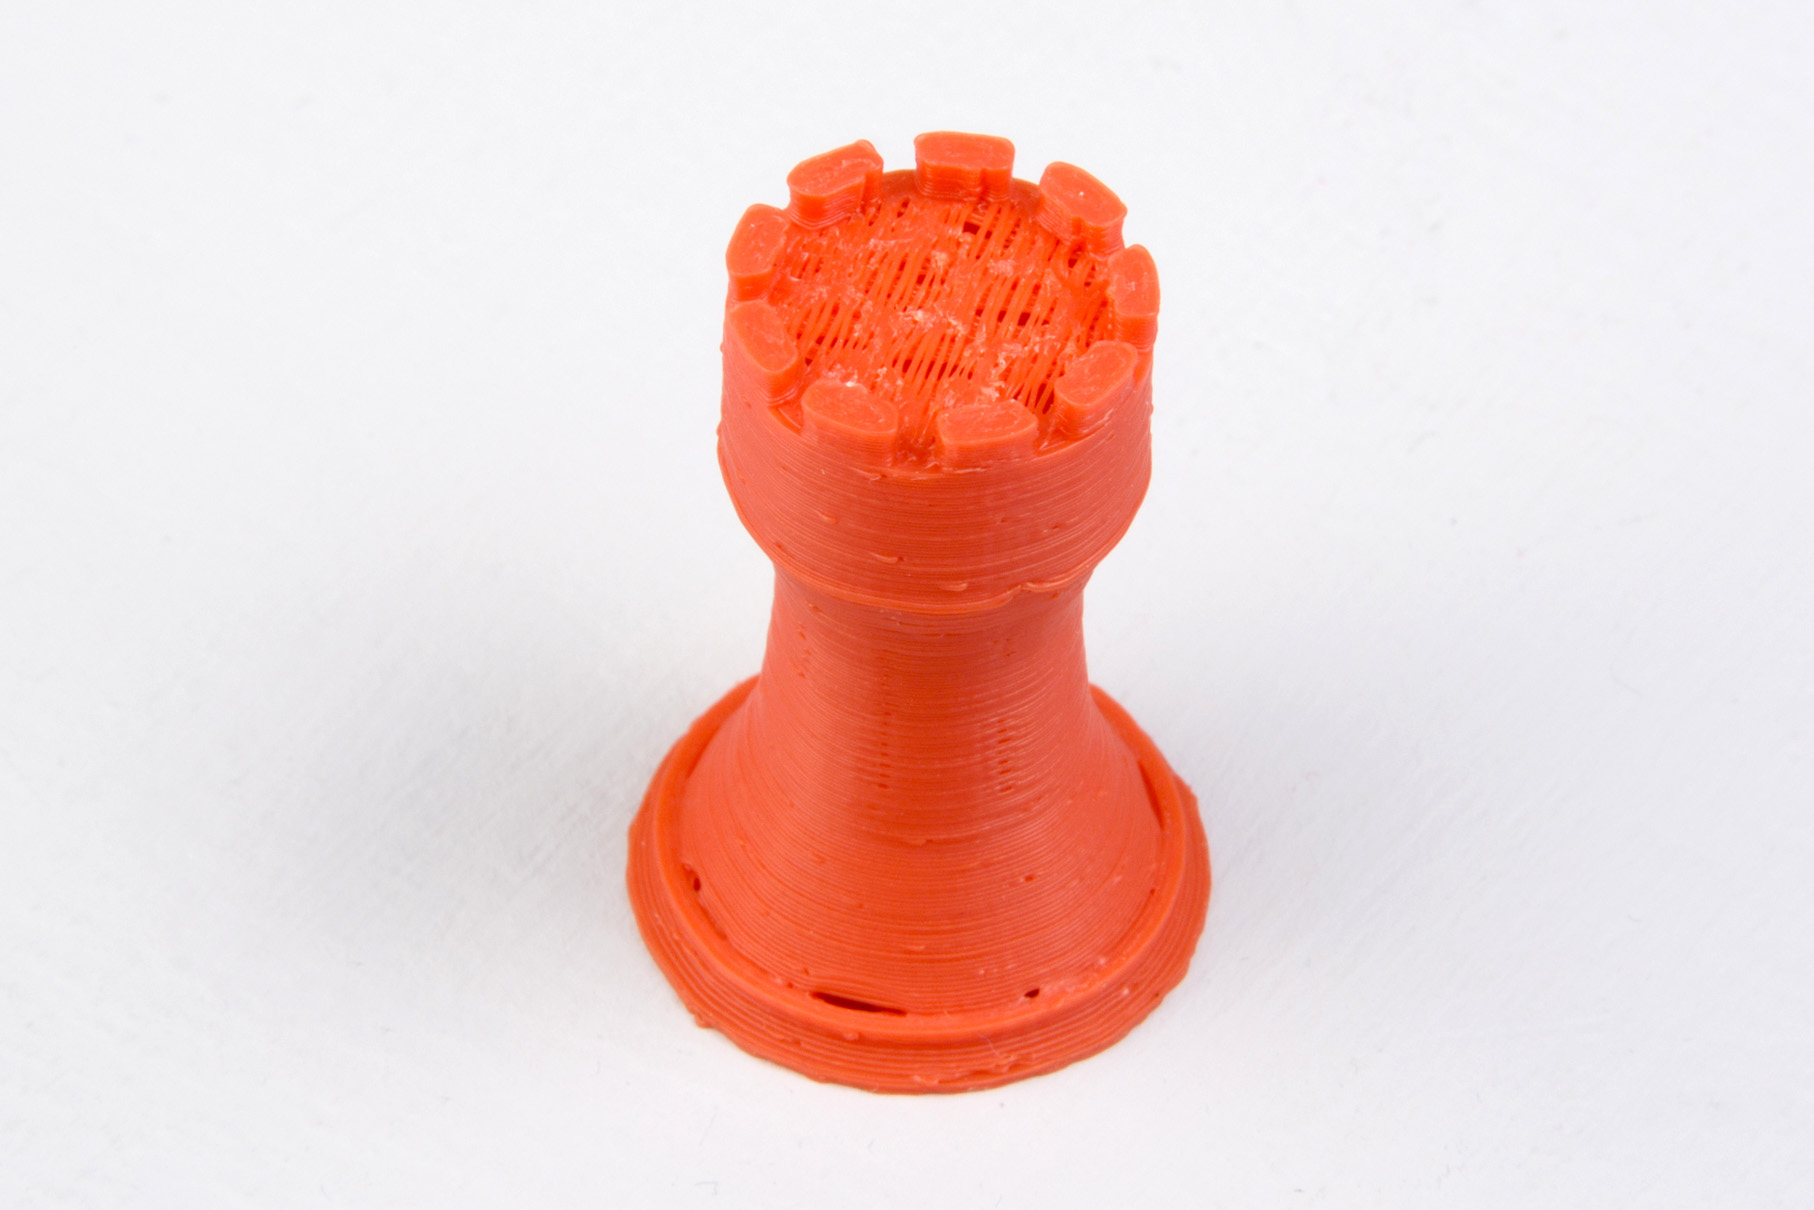
\includegraphics[keepaspectratio=true,width=0.75\textwidth]{simple_mode/bad_top_infill.jpg}
\caption{An example of insufficient top layers.}
\label{fig:bad_top_infill}
\end{figure}

Another tip to consider: Setting the top solid layer to zero, and setting the infill also to zero, will result in a hollow receptacle, ideal for turning models into vases\footnote{http://slic3r.org/blog/tip-printing-vases} for example.  Here manipulating the settings within Slic3r can be used to generate different kinds of prints, and not only be used to control surface accuracy.

\begin{figure}[H]
\centering
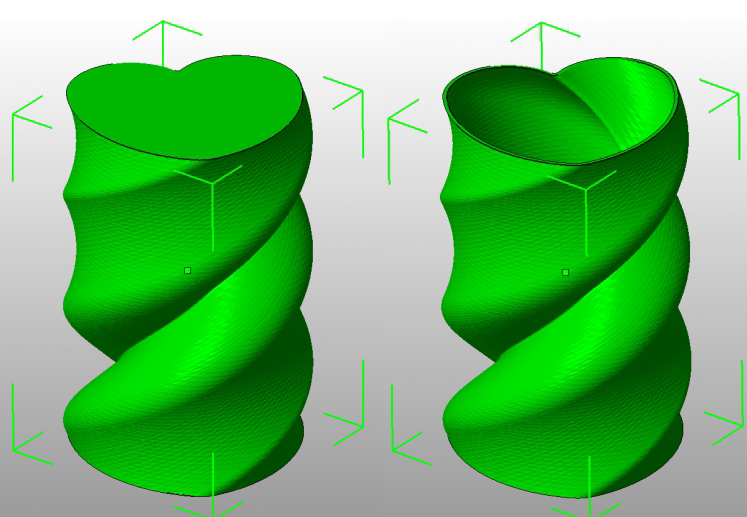
\includegraphics[keepaspectratio=true,width=0.75\textwidth]{simple_mode/solid_layers_vases.png}
\caption{Creating a vase from a solid model.}
\label{fig:solid_layers_vases}
\end{figure}

% paragraph general (end)

\paragraph{Infill.} % (fold)
\label{par:simple_infill}
\index{Print Settings!Infill}
\index{Print Settings!Infill!Fill density}
\texttt{Fill density} is defined on a scale of between 0 and 1, where 1 is 100\% and 0.4 would be 40\%.  For the majority of cases it makes no sense to 100\% fill the model with plastic, this would be a waste of material and take a long time.  Instead, most models can be filled with less material which is then sandwiched between layers filled at 100\% (see \texttt{Solid layers} above).

A density value of 0.4 is enough to give almost all models good mechanical strength.  A value of 0.2 is usually the minimum required to support flat ceilings.

\index{Print Settings!Infill!Fill pattern}
Slic3r offers several fill patterns which will be discussed in more depth in section \ref{sec:infill_patterns_and_density} - Infill Choices.  Choosing a \texttt{Fill pattern} will depend on the kind of model, the desired structural  strength, print speed, and personal taste.  The more exotic fill methods are usually too slow and unnecessarily complex for most use cases, and so most of the time the infill pattern is either \texttt{rectilinear}, \texttt{line}, or \texttt{honeycomb}.  Honeycomb gives the most strength but is slower than both rectilinear or line.

% paragraph infill (end)

\paragraph{Support material.} % (fold)
\label{par:simple_support_material}
\index{Print Settings!Support material}
\index{Print Settings!Support material!Generate support material}
\index{Print Settings!Support material!Pattern spacing}
Printing a model from the bottom up, as with FDM, means that any significant overhangs will be printed in the air, and most likely droop or not print correctly.  Choosing support material (\texttt{Generate support material}) will add additional structures around the model which will build up to then support the overhanging part.  The \texttt{Pattern spacing} option determines how dense the support material is printed.

\begin{figure}[H]
\centering
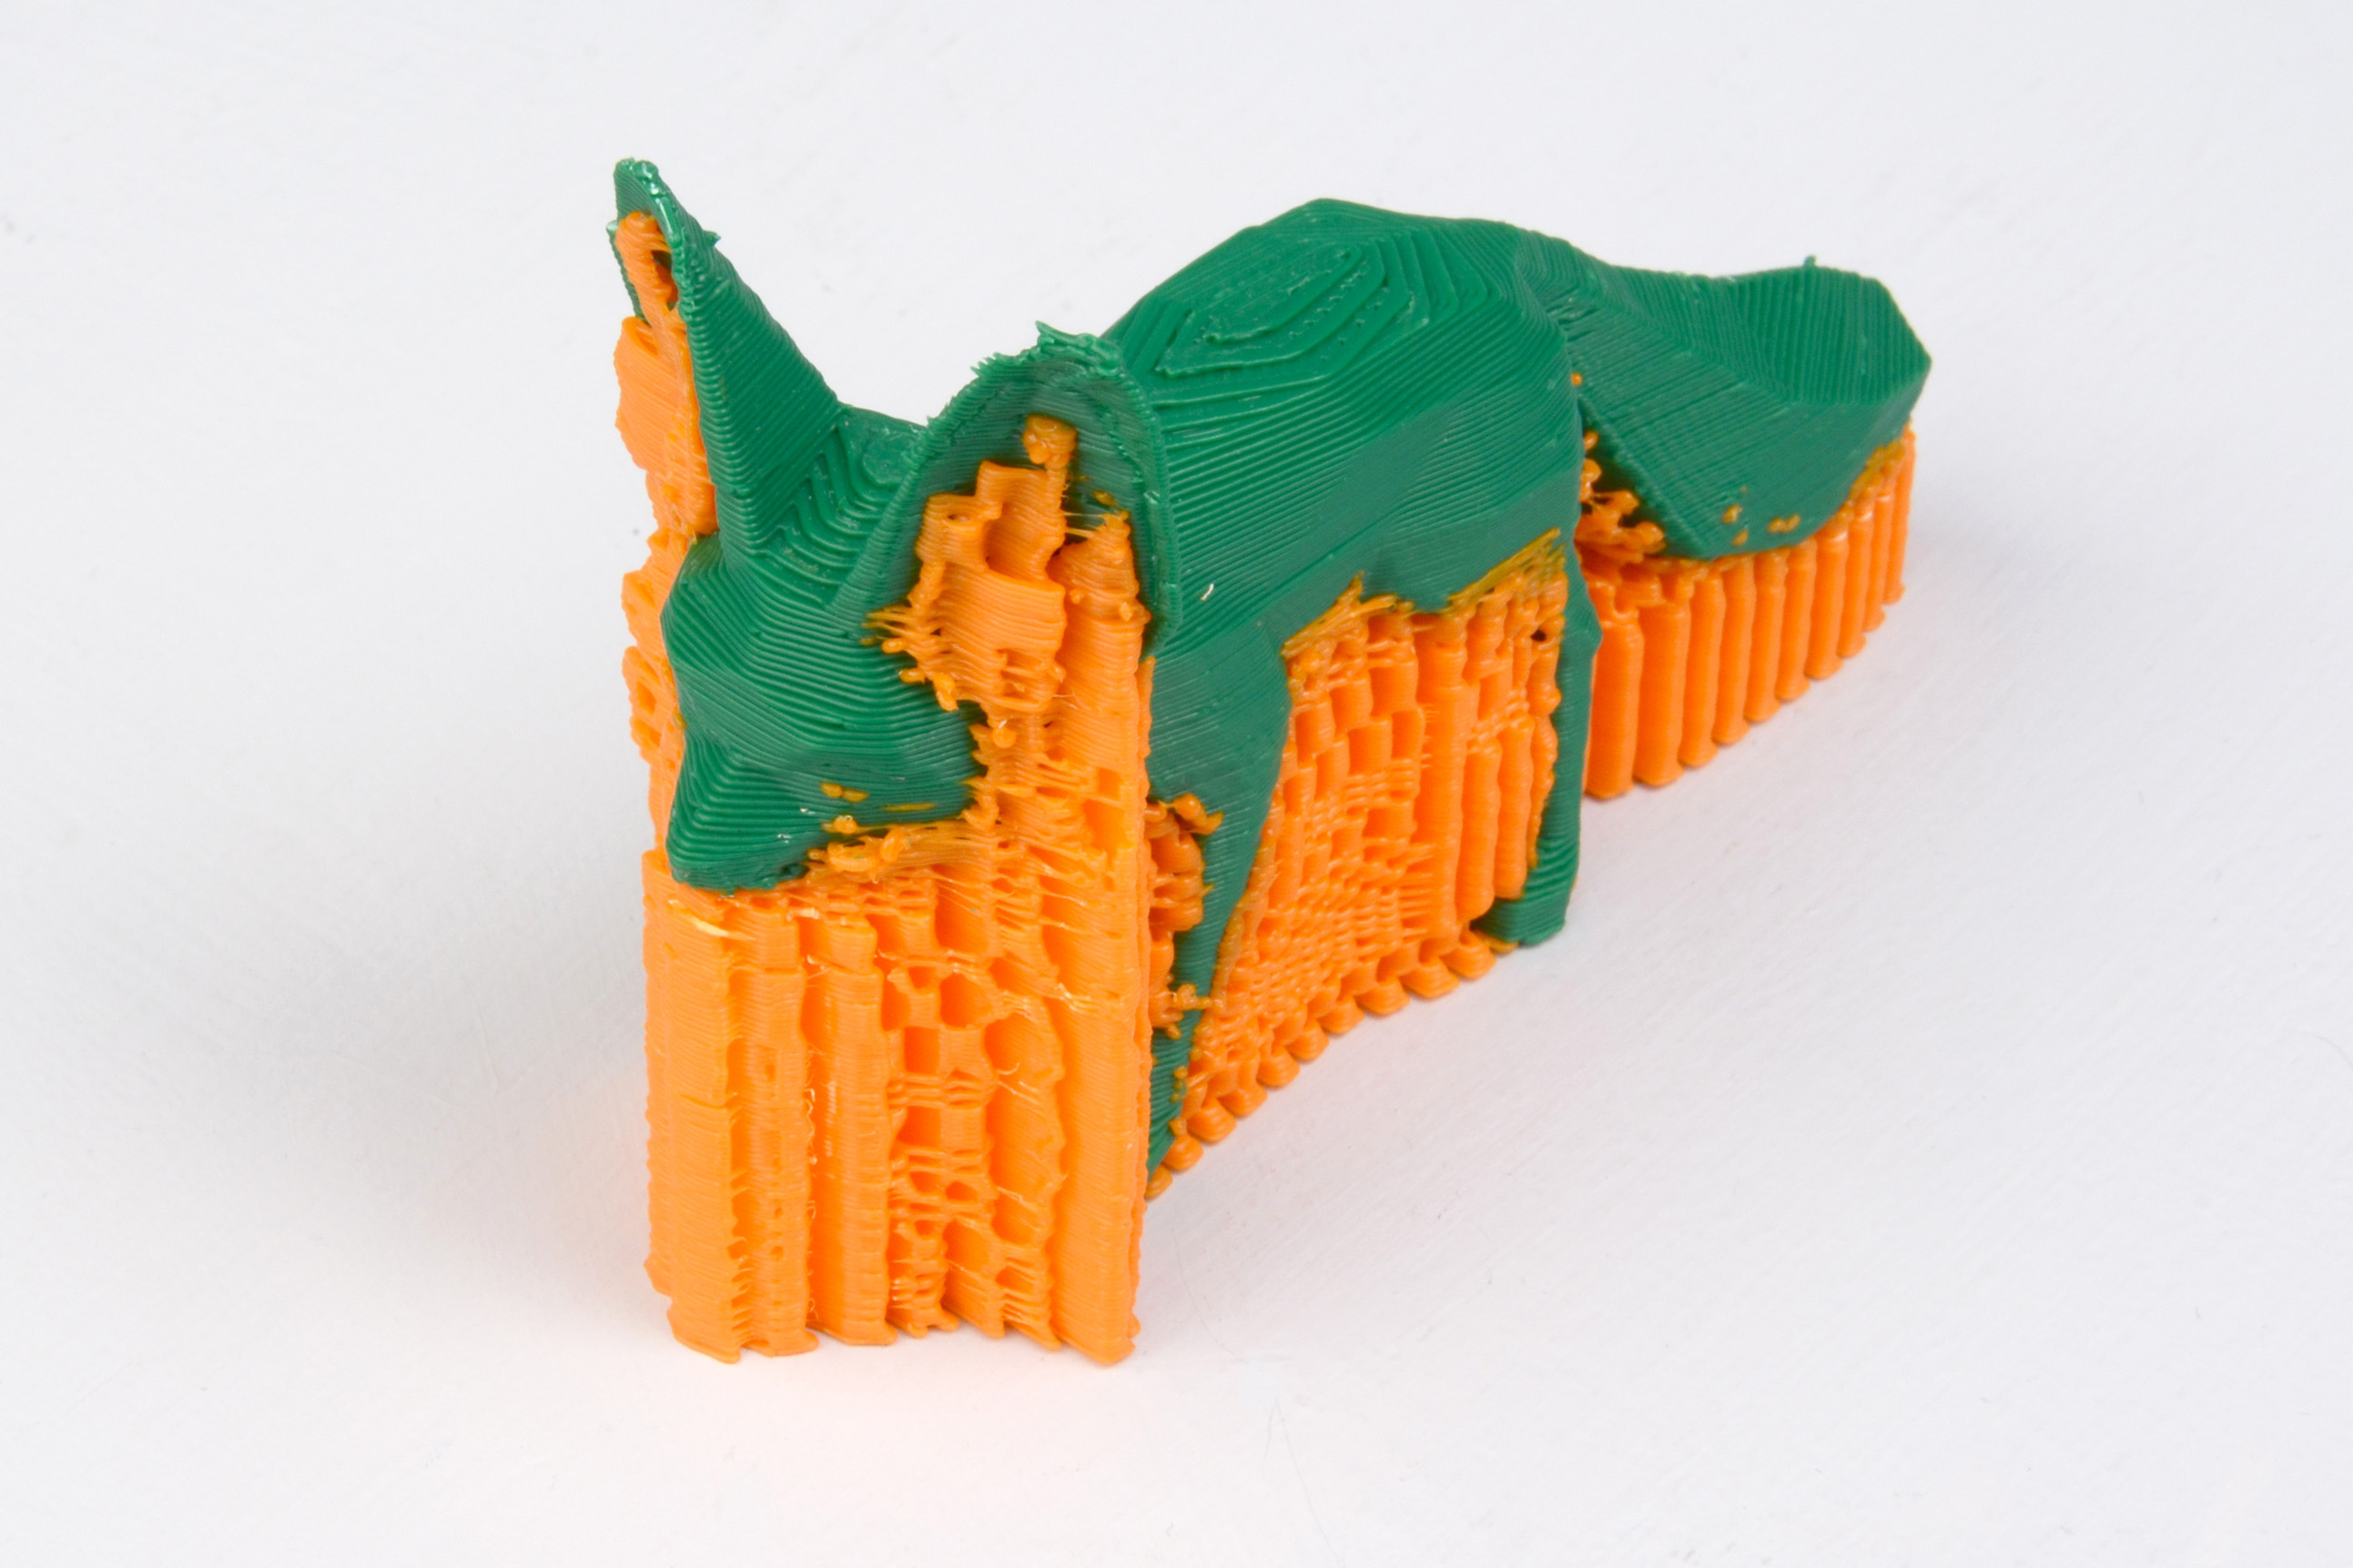
\includegraphics[keepaspectratio=true,width=0.75\textwidth]{simple_mode/support_example.jpg}
\caption{An example of an object printed with support material.}
\label{fig:support_example}
\end{figure}

Tip: It is sometimes worth considering altering the orientation of the model in order to possibly reduce overhangs.

\index{Print Settings!Support material!Raft layers}
\texttt{Raft layers} will add additional layers underneath the model and stems from the early days of 3D printing.  It can help with prints without a heated bed, or where the bed is not very flat, but it is usually not required and is not recommended.  The raft also requires post-processing to remove it.
% paragraph support_material (end)

\paragraph{Speed.} % (fold)
\label{par:simple_speed}
\index{Print Settings!Speed}
In simple mode there are only three speed settings to consider:
\index{Print Settings!Speed!Perimeters}
\index{Print Settings!Speed!Infill}
\index{Print Settings!Speed!Travel}
\begin{itemize}
	\item \texttt{Perimeters}  - The outline of the model may benefit from being printed slightly slower so that the outside skin of the print has fewer blemishes.
	\item \texttt{Infill}  - As the infill is hidden this can be extruded a little faster.  Take care though not to go too fast as higher speeds results in thinner extrusions, and this may affect how the extrusions bond.
	\item \texttt{Travel}  - The jump between the end of one extrusion and the next should usually be performed as quickly as the printer will allow in order to minimise any mess caused by material oozing from the nozzle.
\end{itemize}
% paragraph speed (end)

\paragraph{Brim.} % (fold)
\label{par:simple_brim}
\index{Print Settings!Brim}
\index{Print Settings!Brim!Brim width}
\texttt{Brim width} is used to add more perimeters to the first layer, as a base flange, in order to provide more surface area for the print to stick to the bed with in order to reduce warping (see §\ref{sec:the_important_first_layer}). The brim is then cut away once the print is finished and removed from the bed.

\begin{figure}[H]
\centering
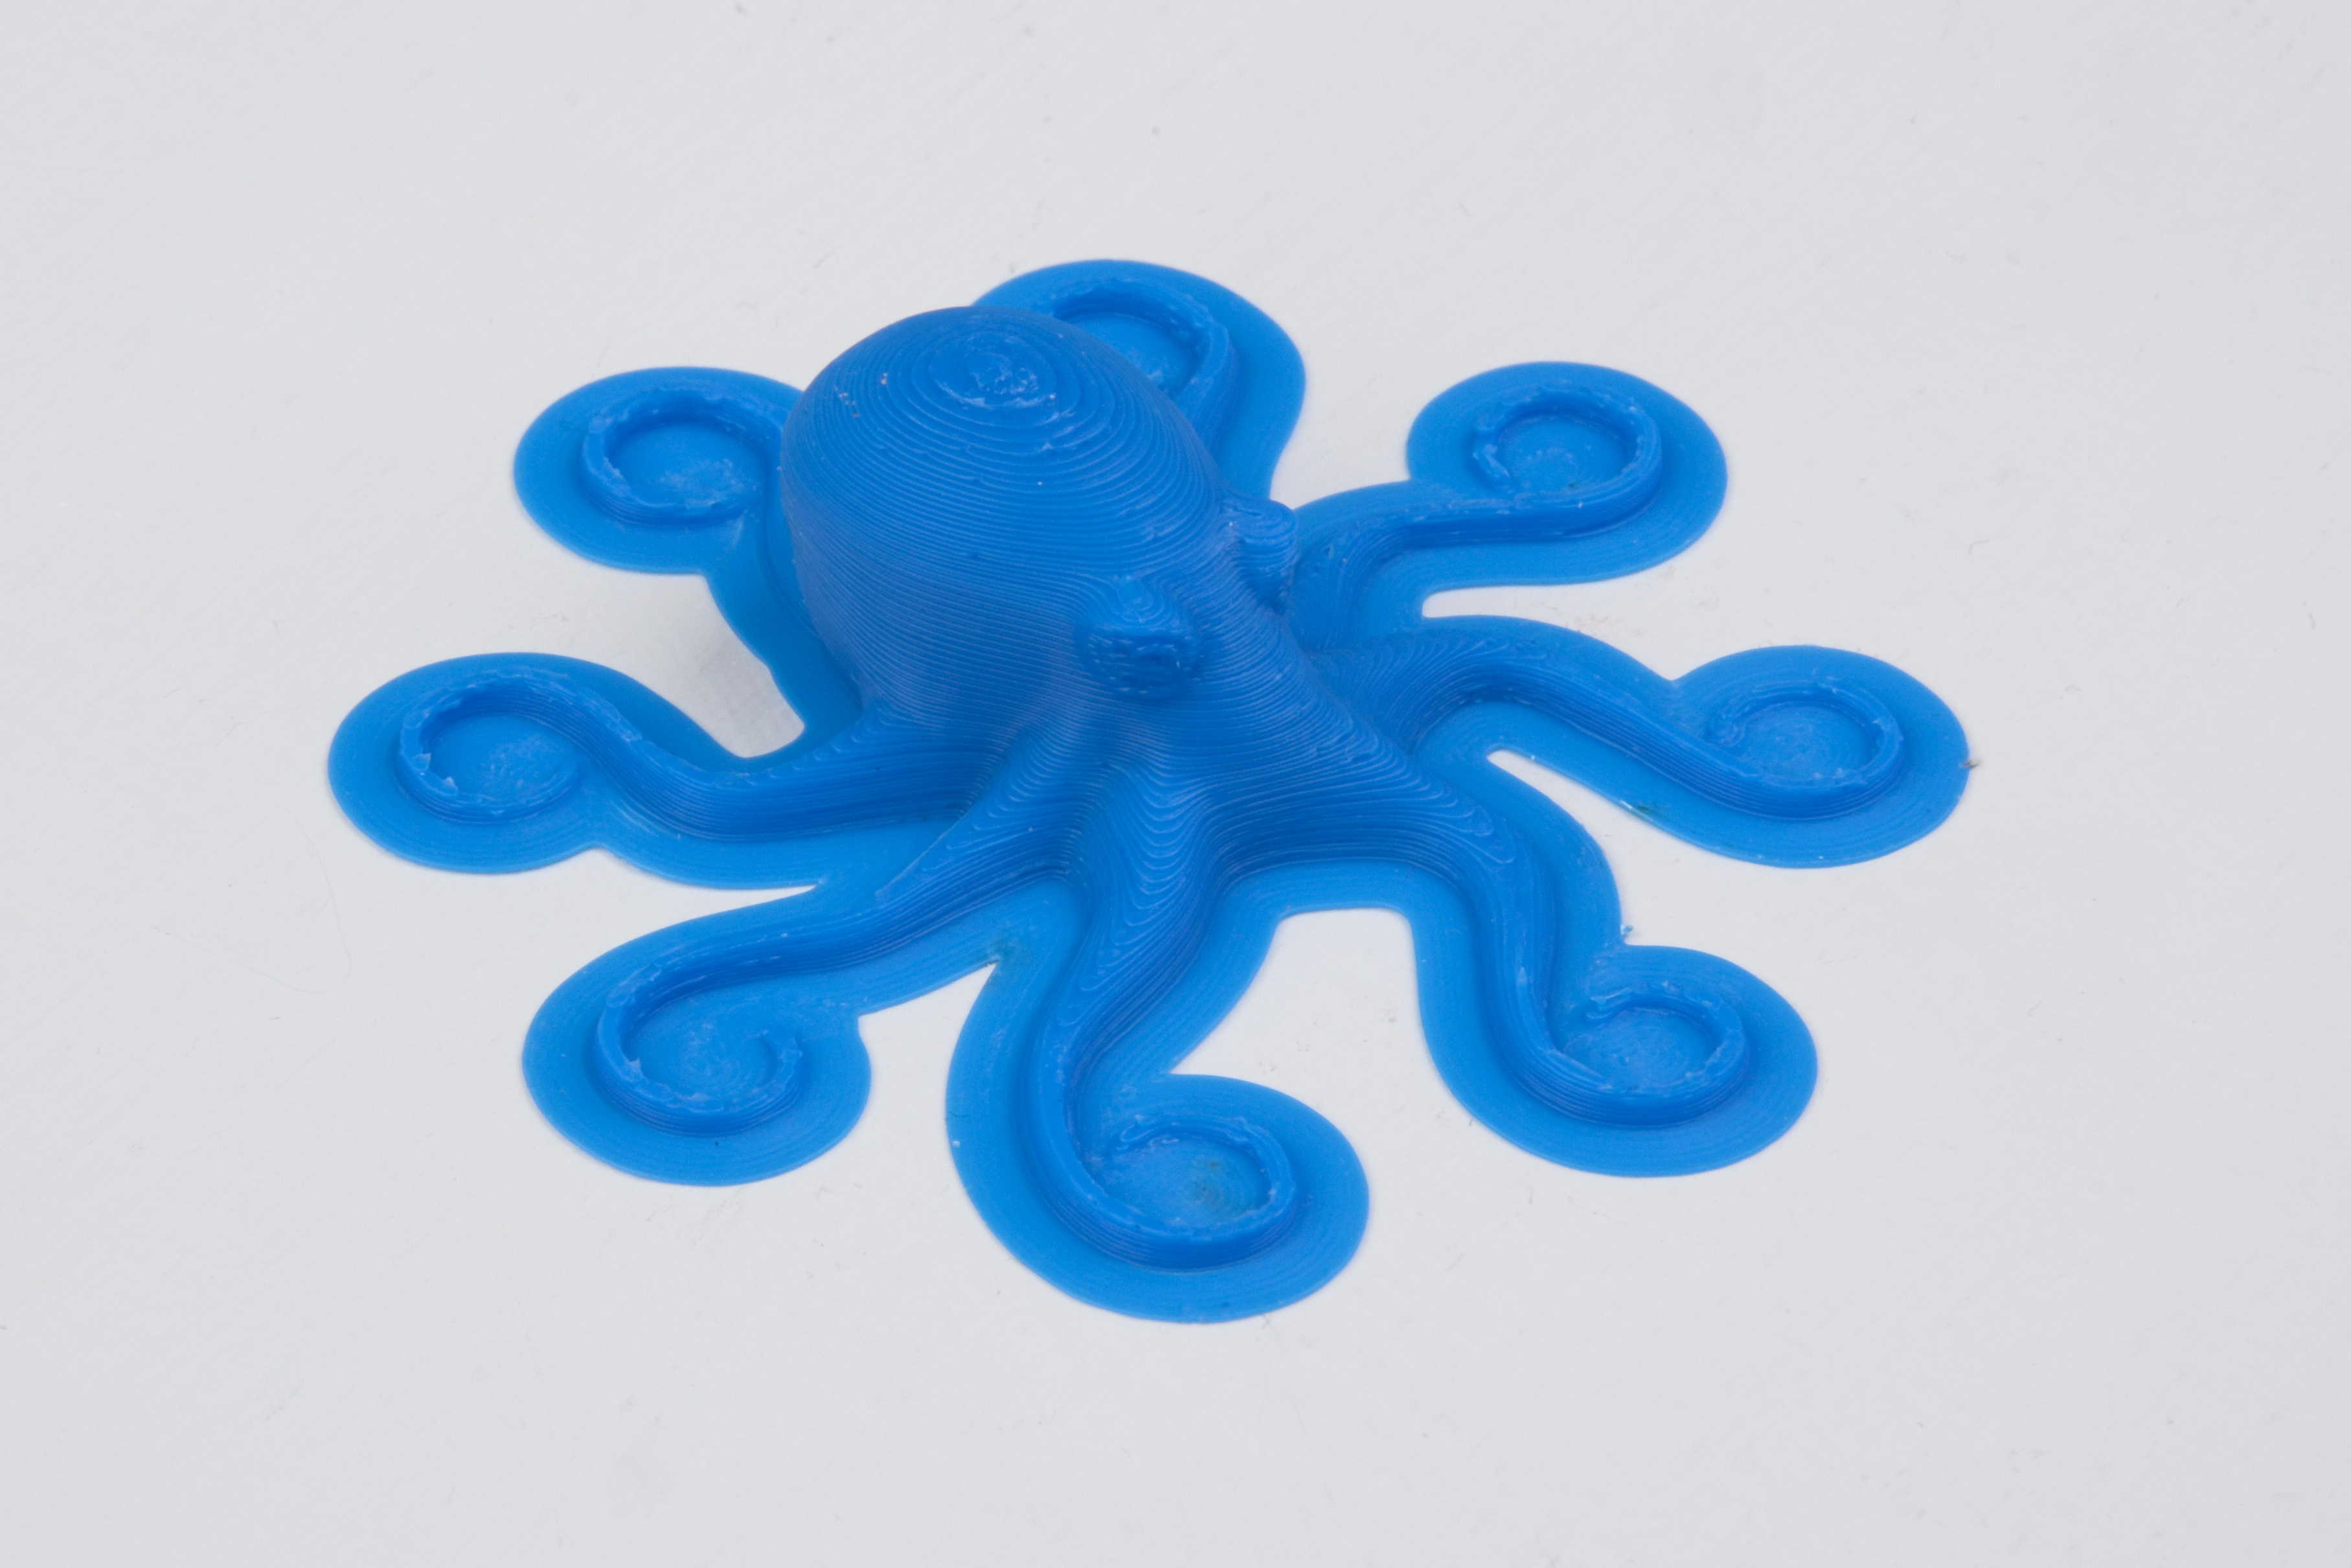
\includegraphics[keepaspectratio=true,width=0.75\textwidth]{simple_mode/brim.jpg}
\caption{An example of brim.}
\label{fig:an_example_of_brim}
\end{figure}

% paragraph brim (end)

\paragraph{Sequential printing.} % (fold)
\label{par:simple_sequential_printing}
\index{Print Settings!Sequential printing}
\index{Print Settings!Sequential printing!Extruder clearance}
When printing several objects at once it can be useful to print each one separately as this will minimise oozing and strings running between the prints.  It will also decrease the risk of a problem ruining the entire print - if one part detaches or fails in some way, it will not be dragged into other parts of the print during each layer.

\begin{figure}[H]
\centering
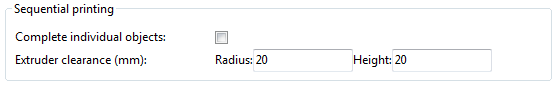
\includegraphics[keepaspectratio=true,width=1\textwidth]{simple_mode/sequential_printing_options.png}
\caption{Sequential printing options.}
\label{fig:sequential_printing_options}
\end{figure}

\index{Print Settings!Sequential printing!Extruder clearance}
Care has to be taken that the nozzle and extruder does not interfere with already printed parts.  Slic3r should warn if it detects the nozzle or extruder will collide with a part, but double check that the layout of the parts will not cause problems.  The \texttt{Extruder clearance} parameters help Slic3r detect potential collisions:
\begin{itemize}
	\item \texttt{Radius}  - The clearance that should be given around the extruder.  Take care if the extruder is not mounted centrally - take the largest safe value.
	\item \texttt{Height}  - The vertical distance between the nozzle tip and the X axis rods, or lowest part which may interfere with a finished print.
\end{itemize}

\begin{figure}[H]
\centering
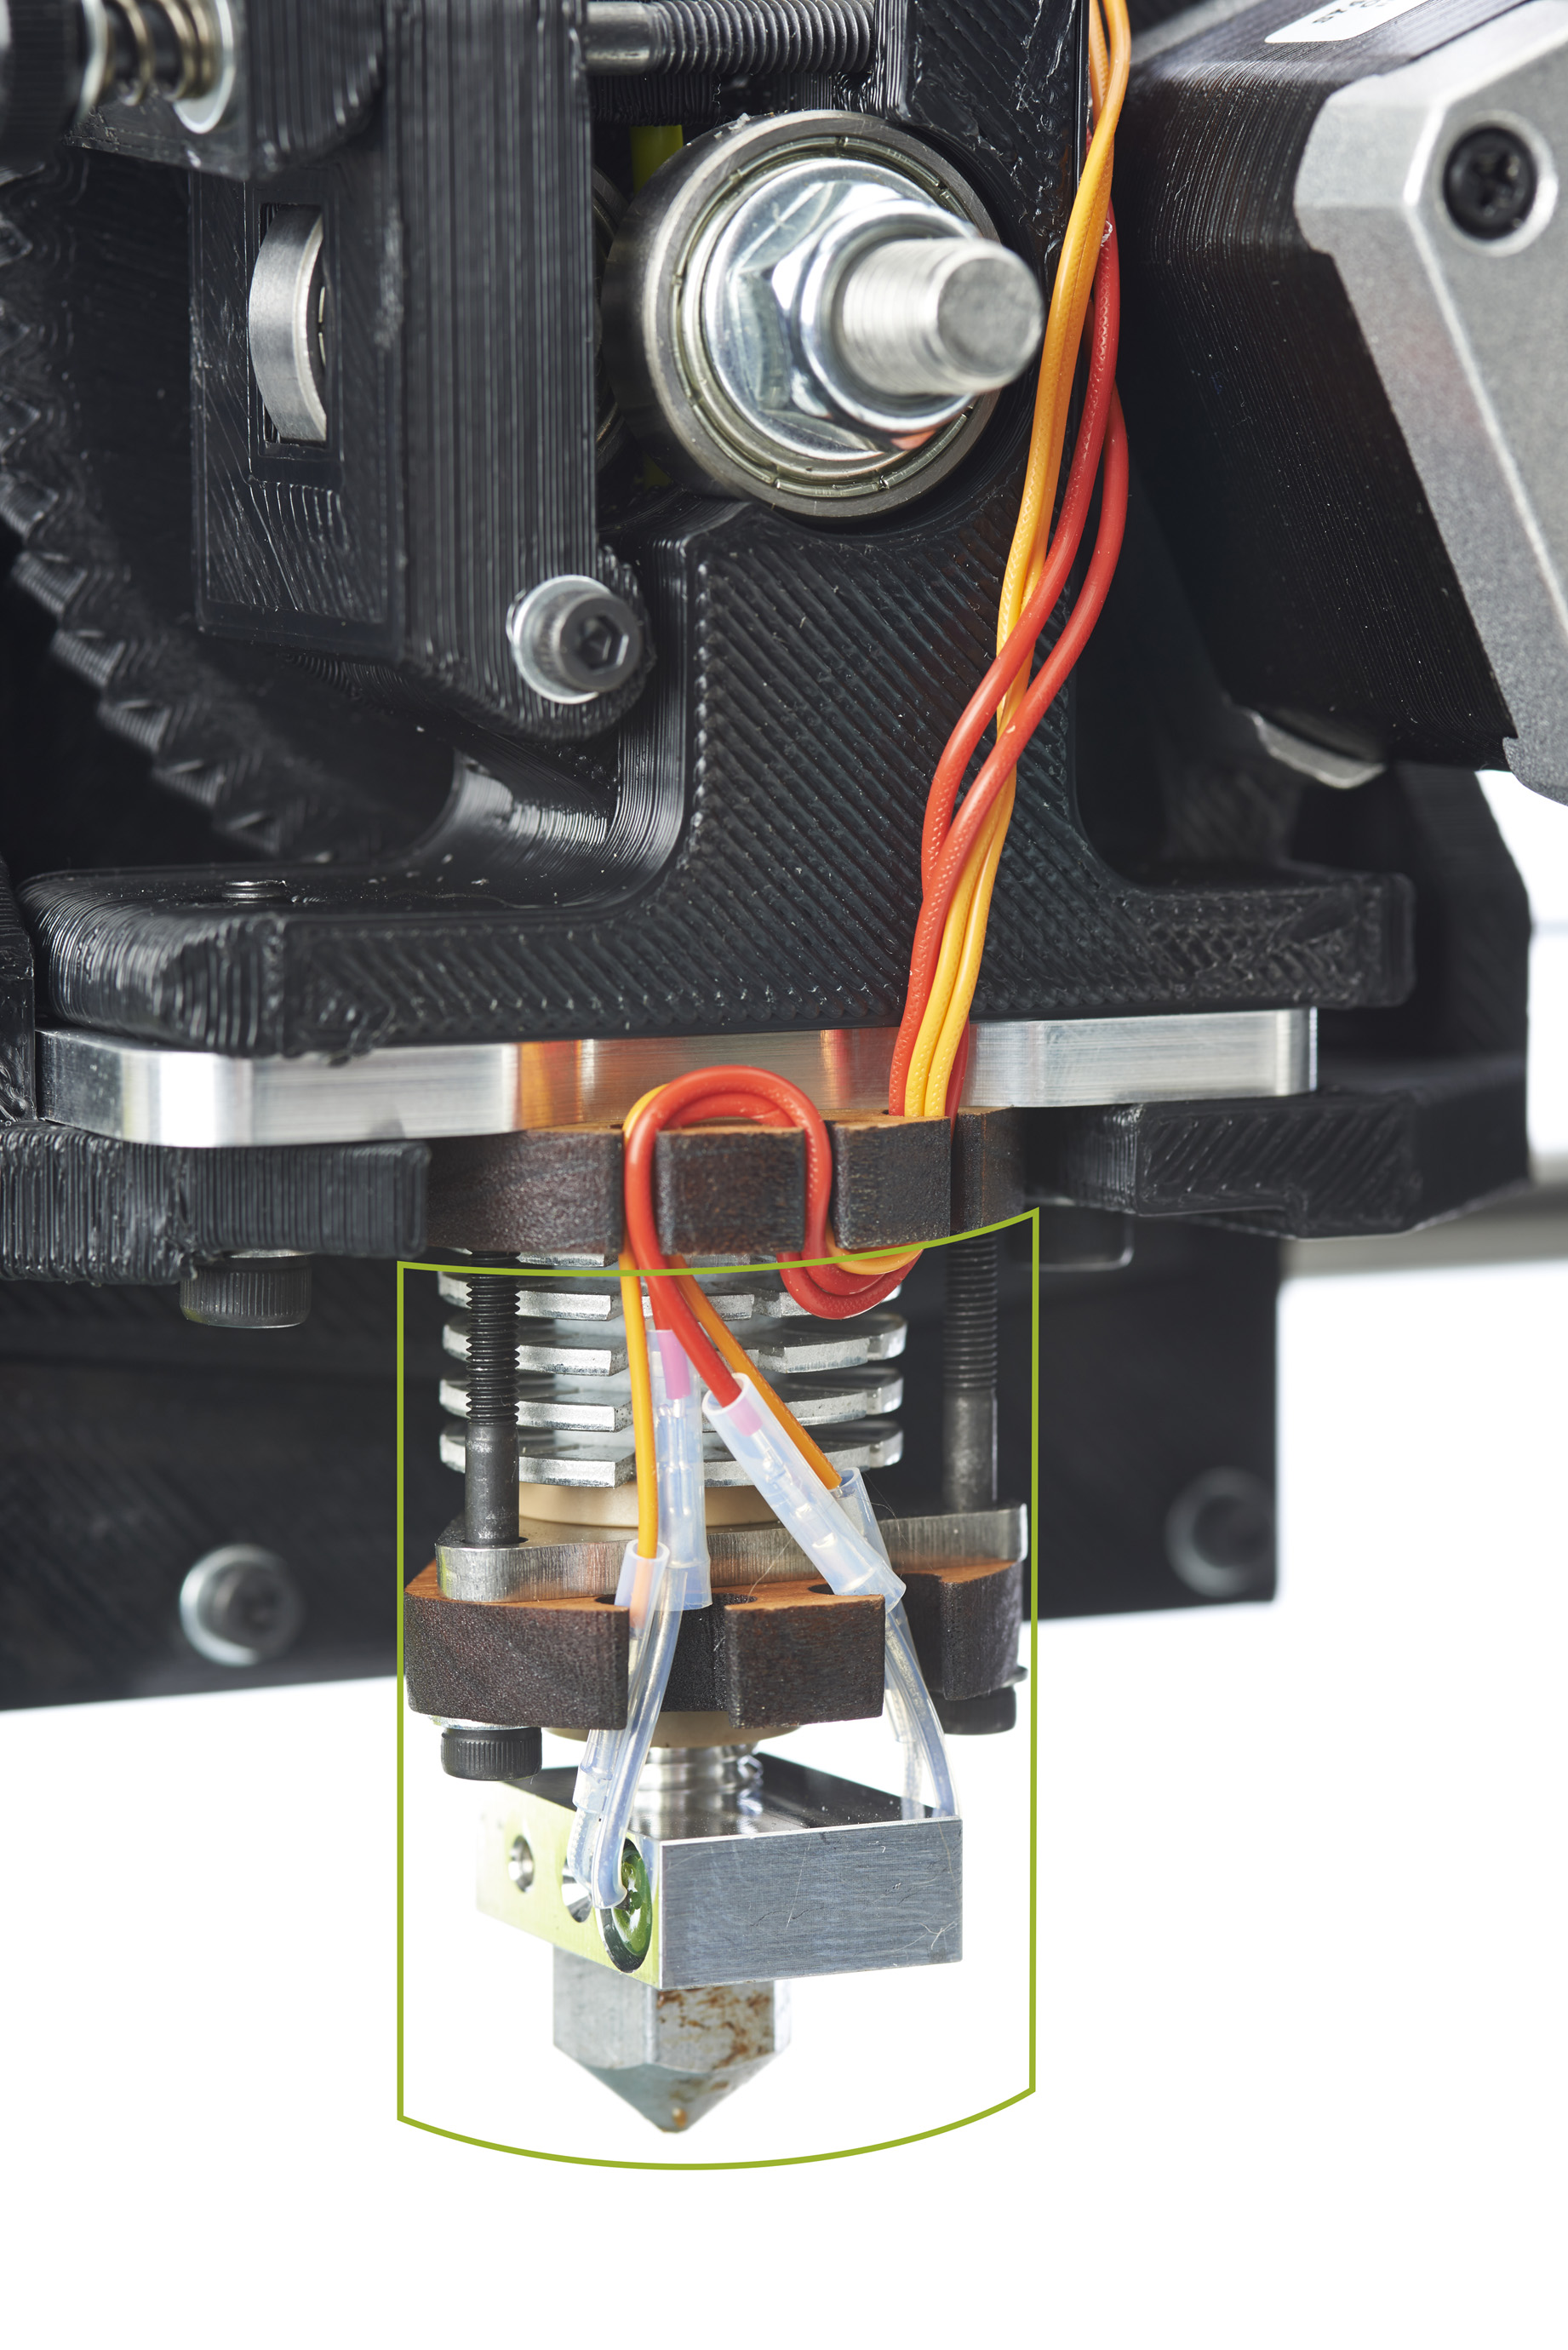
\includegraphics[keepaspectratio=true,width=0.5\textwidth]{simple_mode/extruder_clearance.jpg}
\caption{The clearance cylinder around an extruder.}
\label{fig:a_diagram_depicting_extruder_clearance}
\end{figure}
% paragraph sequential_printing (end)


\subsection{Filament Settings}
\index{Filament Settings}

The \texttt{Filament Settings} will normally be used infrequently, for example on receipt of a new roll of filament.

\begin{figure}[H]
\centering
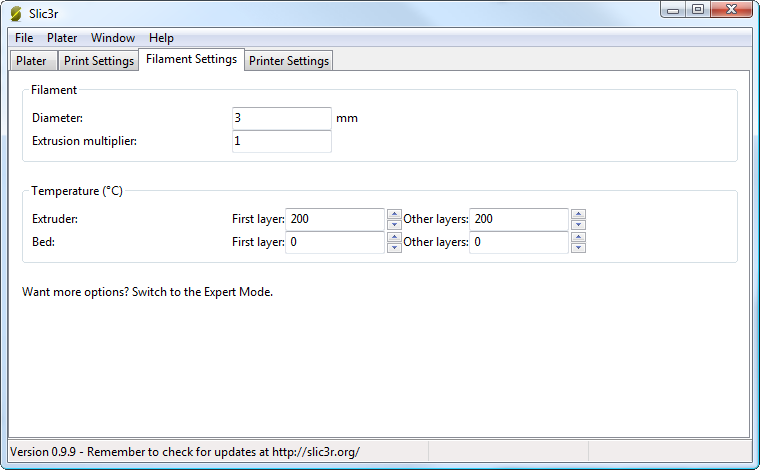
\includegraphics[width=\textwidth]{simple_mode/simple_mode_filament_settings.png}
\caption{Simple Mode: Filament Settings.}
\label{fig:simple_mode_filament_settings}
\end{figure}

\paragraph{Filament.} % (fold)
\label{par:filament}
\index{Filament Settings!Filament}
\index{Filament Settings!Filament!Diameter}
The \texttt{Diameter} setting will already have been filled from the value given during the wizard (see p.\pageref{sub:4_filament_diameter}), but can be updated here.

\index{Filament Settings!Filament!Extrusion multiplier}
The \texttt{Extrusion multiplier} setting allows the fine tuning of the extrusion flow rate, and is is given as a factor, e.g. 1 means 100\%, 1.5 would mean 150\%.  Whilst the value should ideally be set in the firmware it can be useful to test slight changes to the rate by altering this value.  It varies the amount of plastic proportionally and should be changed in very small steps (e.g. +/- 0.05) as the effects are very visible.
% paragraph filament (end)

\paragraph{Temperature.} % (fold)
\label{par:temperature}
\index{Filament Settings!Temperature!Extruder}
\index{Filament Settings!Temperature!Bed}
These values are also filled from the wizard, but here the opportunity exists to set the temperature for the first layer (see p.\pageref{sec:the_important_first_layer}).
% paragraph temperature (end)


\subsection{Printer Settings}
\index{Printer Settings}

The \texttt{Printer Settings} will be updated the least, unless Slic3r is going to be used for many printers, for example, in a 3D printer farm.

\begin{figure}[H]
\centering
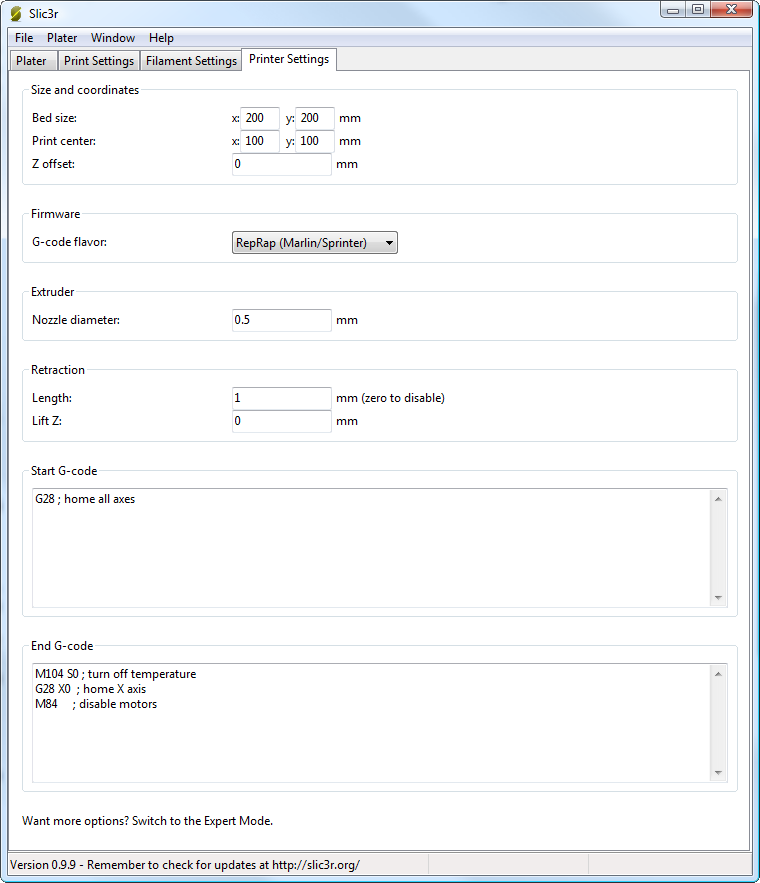
\includegraphics[width=\textwidth]{simple_mode/simple_mode_printer_settings.png}
\caption{Simple Mode: Printer Settings.}
\label{fig:simple_mode_printer_settings}
\end{figure}

\paragraph{Size and coordinates.} % (fold)
\label{par:size_and_coordinates}
\index{Printer Settings!Size and coordinates}
\index{Printer Settings!Size and coordinates!Bed size}
The \texttt{Bed size} setting is taken from the wizard (see p.\pageref{sub:2_bed_size}) and is only used for previewing the model in the plater.

\index{Printer Settings!Size and coordinates!Print center}
The \texttt{Print center} is the point around which the print will be centered.  A \texttt{Bed size} of 200mmx200mm and a \texttt{Print center} of 100mmx100mm would sit the print in the middle.  Should it be desired to print away from the center, because of a scratch in the glass perhaps, then this option should be used.

\index{Printer Settings!Size and coordinates!Z offset}
\texttt{Z offset} can be used to compensate for an incorrectly calibrated Z end-stop.  If the nozzle stops slightly too far from the bed, then adding a negative value will offset all layers by that amount.  The correct solution however is to fix the end-stop itself.

The optimal Z endstop position is where the nozzle tip barely touches the surface of the bed when homed.  A sheet of paper makes a good gauge for this very small distance.  It is not recommended to use this setting to try and improve layer adhesion, by "squashing" the bottom layer into the bed, instead look at the suggestions in section \ref{sec:the_important_first_layer}.
% paragraph size_and_coordinates (end)

\paragraph{Firmware.} % (fold)
\label{par:firmware}
\index{Printer Settings!Firmware!G-code flavour}
As selected in the wizard (see p.\pageref{sub:1_firmware_type}), \texttt{G-code flavour} defines the dialect of G-code generated.
% paragraph firmware (end)


\paragraph{Extruder.} % (fold)
\label{par:extruder}
\index{Printer Settings!Extruder!Nozzle diameter}
\texttt{Nozzle diameter} was defined in the wizard (see p.\pageref{sub:3_nozzle_diameter}).
% paragraph extruder (end)

\paragraph{Retraction.} % (fold)
\label{par:retraction}
\index{Printer Settings!Extruder!Retraction!Length}
Unless the material being extruded has a very high viscosity it may ooze between extrusions due to gravity.  This can be remedied by actively retracting the filament between extrusions.  Setting the \texttt{Length} parameter to a positive value will cause the filament to be reversed by that many millimeters before travel.  The retraction will then be compensated for by the same amount after the travel move, before starting the new extrusion path.

A value of between 1 and 2mm is usually recommended. Bowden extruders may need up to 4 or 5mm due to the hysteresis introduced by the tube.
\index{Printer Settings!Extruder!Retraction!Lift Z}
Setting the \texttt{Lift Z} parameter to a positive value will raise the entire extruder on the Z axis by that many millimeters during each travel.  This can be useful to ensure the nozzle will not catch on any already laid filament, however it is usually not necessary and will slow the print speed.  A value of 0.1mm is usually sufficient.
% paragraph retraction (end)

\paragraph{Start, End and Layer Chance G-codes.} % (fold)
\label{par:start_end_g_code}
\index{Printer Settings!Custom G-code!Start G-code}
\index{Printer Settings!Custom G-code!End G-code}
Custom G-code commands can be run before a print starts and after a print finishes.

Placeholders can be inserted in the G-code commands\footnote{https://github.com/alexrj/Slic3r/wiki/FAQ\#what-placeholders-can-i-use-in-custom-g-code}.  For example [next\_extruder] would return the index of the next extruder.

The RepRap wiki is a good resource to learn about the variety of G-codes available: \texttt{http://reprap.org/wiki/G-code}.

Note: Be sure to check that a given G-code is valid for your firmware.

The codes specified in \texttt{Start G-code} are inserted at the beginning of the output file, directly after the temperature control commands for extruder and bed.  Note that if temperature control commands are specified (M104 and M190) then these will replace the temperature G-codes introduced by the \texttt{Filament} settings.

Some common G-codes to use before the print starts are:
\begin{itemize}
	\item \textbf{G28}  - Homes all the axes.
\end{itemize}


Some common G-codes to use after the print ends are:
\begin{itemize}
	\item \textbf{M104 S0}  - Sets the extruder temperature to zero.
	\item \textbf{M140 S0} - Sets the heated bed temperature to zero.
	\item \textbf{G28 X0} - Home the X axis.
	\item \textbf{M84}  - Disables the motors.
\end{itemize}
% paragraph start_end_g_code (end)

% section simple_mode (end)\section{Simple Mode}
